%%%%%%%%%%%%%%%%%%%%%%%%%%%%%%%%%%%%%%%%%
% Short Sectioned Assignment LaTeX Template Version 1.0 (5/5/12)
% This template has been downloaded from: http://www.LaTeXTemplates.com
% Original author:  Frits Wenneker (http://www.howtotex.com)
% License: CC BY-NC-SA 3.0 (http://creativecommons.org/licenses/by-nc-sa/3.0/)
%%%%%%%%%%%%%%%%%%%%%%%%%%%%%%%%%%%%%%%%%

%----------------------------------------------------------------------------------------
%	PACKAGES AND OTHER DOCUMENT CONFIGURATIONS
%----------------------------------------------------------------------------------------

\documentclass[paper=a4, fontsize=11pt]{scrartcl} % A4 paper and 11pt font size

% ---- Entrada y salida de texto -----

\usepackage[T1]{fontenc} % Use 8-bit encoding that has 256 glyphs
\usepackage[utf8]{inputenc}
%\usepackage{fourier} % Use the Adobe Utopia font for the document - comment this line to return to the LaTeX default

% ---- Idioma --------

\usepackage[spanish, es-tabla]{babel} % Selecciona el español para palabras introducidas automáticamente, p.ej. "septiembre" en la fecha y especifica que se use la palabra Tabla en vez de Cuadro

% ---- Otros paquetes ----

\usepackage{url} % ,href} %para incluir URLs e hipervínculos dentro del texto (aunque hay que instalar href)
\usepackage{amsmath,amsfonts,amsthm} % Math packages
%\usepackage{graphics,graphicx, floatrow} %para incluir imágenes y notas en las imágenes
\usepackage{graphics,graphicx, float} %para incluir imágenes y colocarlas

\usepackage{listings}	%para incluir remarcado para comandos bash

% Para hacer tablas comlejas
%\usepackage{multirow}
%\usepackage{threeparttable}

%\usepackage{sectsty} % Allows customizing section commands
%\allsectionsfont{\centering \normalfont\scshape} % Make all sections centered, the default font and small caps

\usepackage{fancyhdr} % Custom headers and footers
\pagestyle{fancyplain} % Makes all pages in the document conform to the custom headers and footers
\fancyhead{} % No page header - if you want one, create it in the same way as the footers below
\fancyfoot[L]{} % Empty left footer
\fancyfoot[C]{} % Empty center footer
\fancyfoot[R]{\thepage} % Page numbering for right footer
\renewcommand{\headrulewidth}{0pt} % Remove header underlines
\renewcommand{\footrulewidth}{0pt} % Remove footer underlines
\setlength{\headheight}{13.6pt} % Customize the height of the header

\numberwithin{equation}{section} % Number equations within sections (i.e. 1.1, 1.2, 2.1, 2.2 instead of 1, 2, 3, 4)
\numberwithin{figure}{section} % Number figures within sections (i.e. 1.1, 1.2, 2.1, 2.2 instead of 1, 2, 3, 4)
\numberwithin{table}{section} % Number tables within sections (i.e. 1.1, 1.2, 2.1, 2.2 instead of 1, 2, 3, 4)

\setlength\parindent{0pt} % Removes all indentation from paragraphs - comment this line for an assignment with lots of text

\newcommand{\horrule}[1]{\rule{\linewidth}{#1}} % Create horizontal rule command with 1 argument of height

\usepackage{booktabs}
\usepackage{tabularx}
\usepackage{multicol} 
\usepackage{hyperref}

%----------------------------------------------------------------------------------------
%	TÍTULO Y DATOS DEL ALUMNO
%----------------------------------------------------------------------------------------

\title{
\normalfont \normalsize 
\textsc{\textbf{Ingeniería del conocimiento (2020-2021)} \\ Máster en ingeniería informática \\ Universidad de Granada} \\ [25pt] % Your university, school and/or department name(s)
\horrule{0.5pt} \\[0.4cm] % Thin top horizontal rule
\huge Práctica 1: Desarrollo de un Sistema de
Recuperación de Información con Lucene \\ % The assignment title
\horrule{2pt} \\[0.5cm] % Thick bottom horizontal rule
}
\author{Manuel Orantes Taboada \\ \\ manuelorantes96@gmail.com \\ morantes96@correo.ugr.es \\ 77150692K} % Nombre y apellidos

\date{\normalsize\today} % Incluye la fecha actual

%----------------------------------------------------------------------------------------
% DOCUMENTO
%----------------------------------------------------------------------------------------

\begin{document}

\maketitle % Muestra el Título

\newpage %inserta un salto de página

\tableofcontents % para generar el índice de contenidos

\newpage

\section{Descripción}

En la práctica, el objetivo era realizar un sistema de recuperación con Lucene. Para ello se han desarrollado dos aplicaciones. La primera aplicación se trata del indexador, que crea a partir de una colección de documentos un conjunto de índices que permitan más tarde realizar una búsqueda a través de ellos. El segundo programa es un buscador, que recibe como argumento el conjunto de índices creado anteriormente. Además, es una aplicación con interfaz gráfica, por lo que no es necesario pasar por terminal la búsqueda a realizar.\\

En primer lugar, comentar los archivos que elegí como documentos de mi sistema. Es un conjunto de 157 documentos obtenidos de los enlaces que se predisponían desde la práctica. La colección es: \url{https://kdd.ics.uci.edu/databases/nsfabs/nsfawards.html} - Parte1 - Premios 1994 - Awd\_1994\_61 . La colección hace referencia a abstract premiados por distintos tipos de búsquedas (búsqueda básica, bolsa de palabras, búsqueda indexada...).\\ 

\subsection{Indexador}
Para realizar la primera aplicación, he seguido tanto los pasos del esbozo de la práctica como unos tutoriales por internet, que al fin y al cabo, solo distan entre sí del hecho de que unos son más actuales y con versiones más recientes de lucene. Los pasos a seguir fueron:

\begin{itemize}
	\item Crear un filtro para los archivos.
	El conjunto de los documentos que elegí, tiene dentro de este un archivo .html con la dirección de cada uno de ellos, y esto no resultaba interesante para el proyecto. Con el filtro, solo proceden a ser indexados los archivos .txt .
	\item Uso de constantes globales para definir donde se encuentran los archivos.
	\item Crear el indexador en sí, y para ello:
	\begin{itemize}
		\item Creamos un indexador con un Analizador al que previamente le hemos introducido nuestra serie de palabras vacías.
		\item Abrimos el fichero en donde están los documentos.
		\item Pasamos el indexador documento por documento.
	\end{itemize}
\end{itemize}

A continuación vemos una ejecución por terminal del indexador junto a los archivos que genera:\\

Para usarlo, simplemente hay que ejecutar el .jar junto con un argumento, que será el directorio en el cual están los documentos:

\begin{figure}[H]
	\centering
	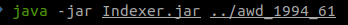
\includegraphics[width=0.4\linewidth]{Imagenes/screenshot001}
	\label{fig:screenshot001}
\end{figure}

En este caso, mi directorio estaba en la carpeta previa a donde estaba el .jar . Una vez se ejecuta, podemos ver como empieza a cargar los ficheros del directorio y comienza a indexarlos uno a uno:

\begin{figure}[H]
	\centering
	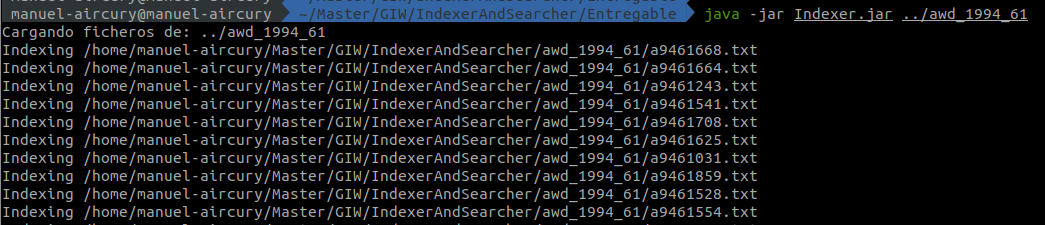
\includegraphics[width=1\linewidth]{Imagenes/screenshot002}
	\label{fig:screenshot002}
\end{figure}

Como resultado, obtenemos en el directorio en el que se encuentra nuestro .jar otra carpeta llamada Indices, que muestra el siguiente contenido:

\begin{figure}[H]
	\centering
	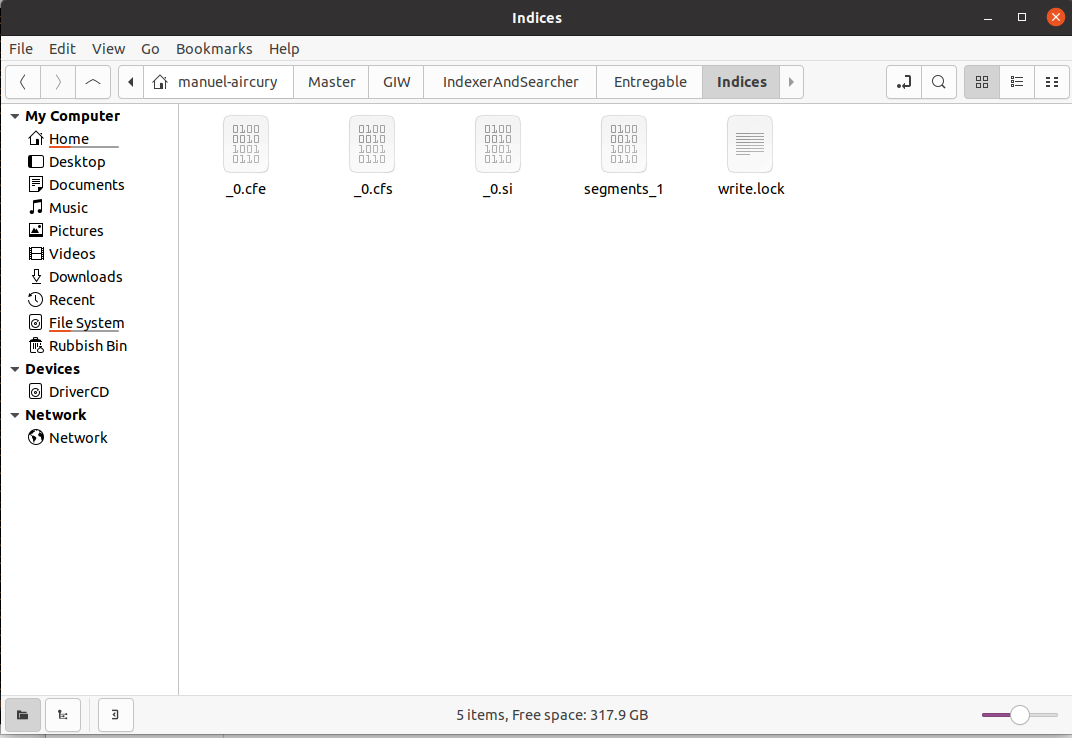
\includegraphics[width=0.7\linewidth]{Imagenes/screenshot003}
	\label{fig:screenshot003}
\end{figure}

Ya estarían los índices preparados para que más tarde el buscador los utilice.\\

Hay que subrayar que intenté un visualizado de estos índices mediante Luke pero me salía que las versiones no eran compatibles, así que no he podido adjuntar imágenes de estos índices.

\newpage
\subsection{Buscador}

Para la segunda aplicación, al igual que en la primera, seguí los pasos tanto de la práctica como de otros tutoriales. Esta vez, los pasos a seguir son los siguientes:
\begin{itemize}
	\item Obtener un buscador a través de índices con Lucene.
	\item Aplicar las medidas pertinentes a la búsqueda introducida.
	\item Obtener los resultados del buscador, que serán los archivos encontrados.
\end{itemize}

Además, también se vieron diferentes vídeos para recordar como era crear una aplicación con Java, para poder buscar por ella, obtener los resultados y podre abrir los ficheros.\\

Para usar la aplicación, al igual que antes, ejecutaremos el .jar desde la línea de comandos junto con el conjunto de índices a usar. En este caso, usaremos los índices que hemos obtenido a través de la primera aplicación:

\begin{figure}[H]
	\centering
	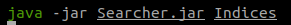
\includegraphics[width=0.4\linewidth]{Imagenes/screenshot004}
	\label{fig:screenshot004}
\end{figure}

Esto nos abrirá una interfaz, en la que encontramos un campo de texto en el cual podemos escribir junto con un botón para realizar la búsqueda:

\begin{figure}[H]
	\centering
	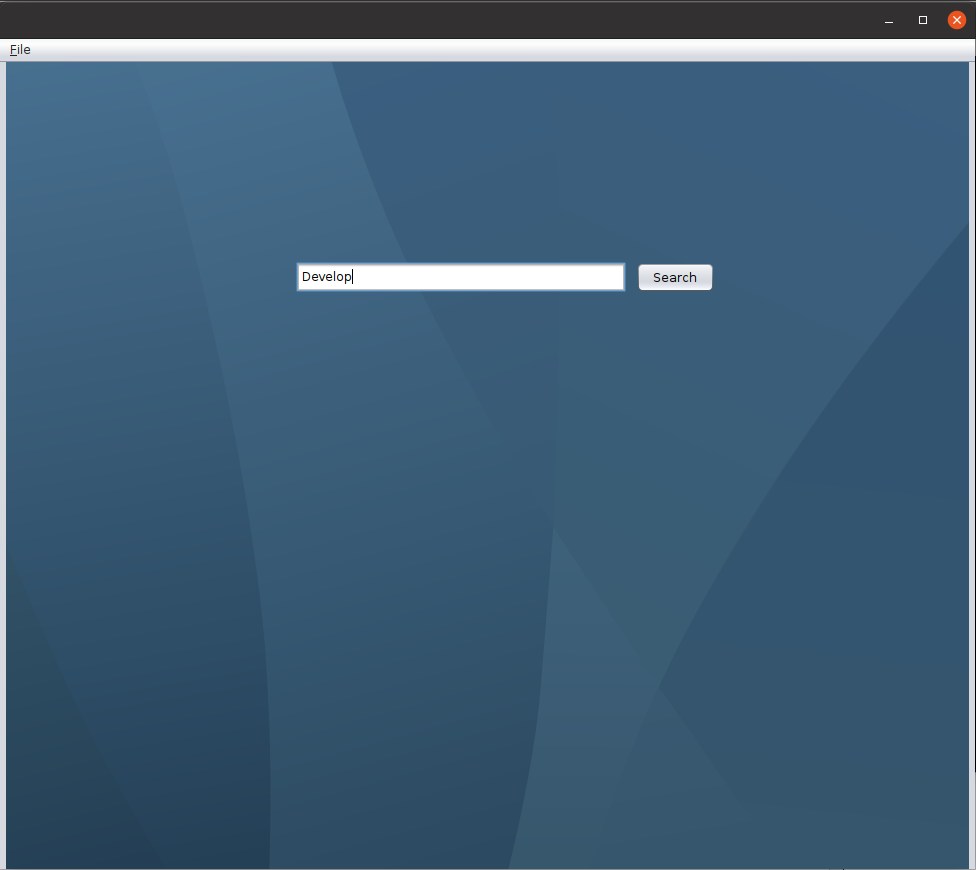
\includegraphics[width=0.7\linewidth]{Imagenes/screenshot005}
	\label{fig:screenshot005}
\end{figure}

Cuando le demos al botón de buscar, se nos abrirá otra pestaña en la cual encontraremos 10 botones junto con un número del 1 al 10, indicando dicho número qué documento se adecua más a nuestra búsqueda:

\begin{figure}[H]
	\centering
	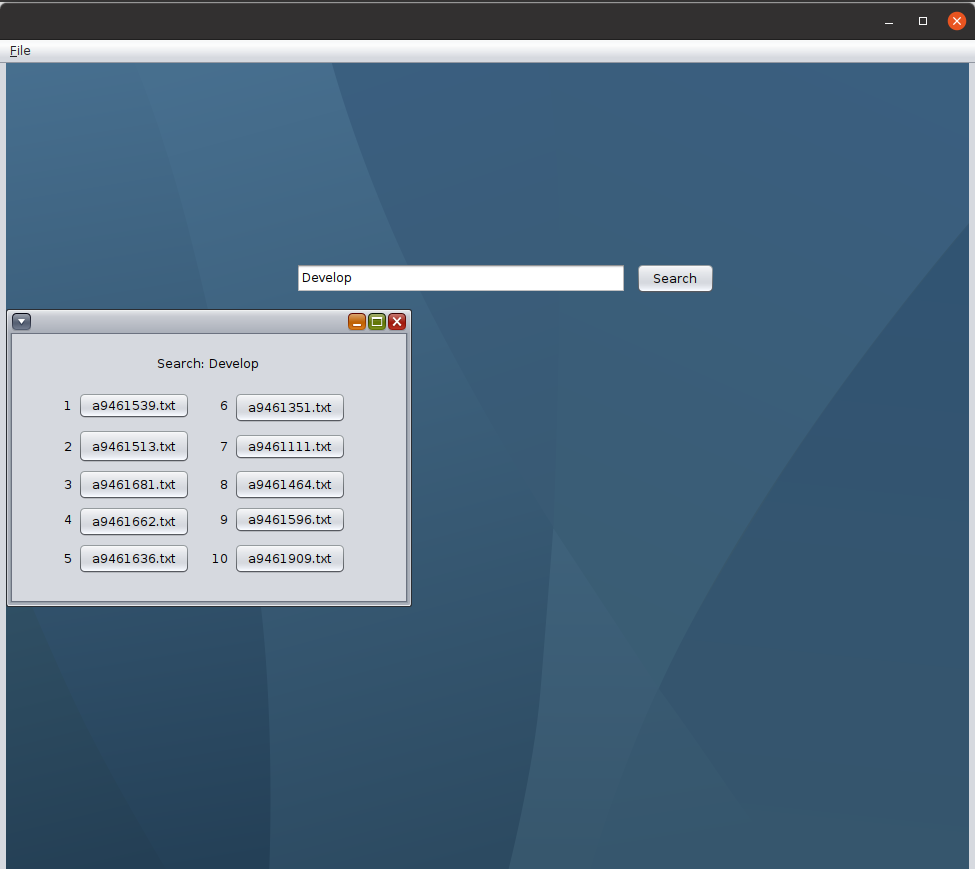
\includegraphics[width=0.7\linewidth]{Imagenes/screenshot006}
	\label{fig:screenshot006}
\end{figure}

Además, podemos realizar varias búsquedas sin cerrar esta pestaña, y podremos diferenciarlas gracias a un etiqueta que nos indica a qué búsqueda pertenecen los archivos:


\begin{figure}[H]
	\centering
	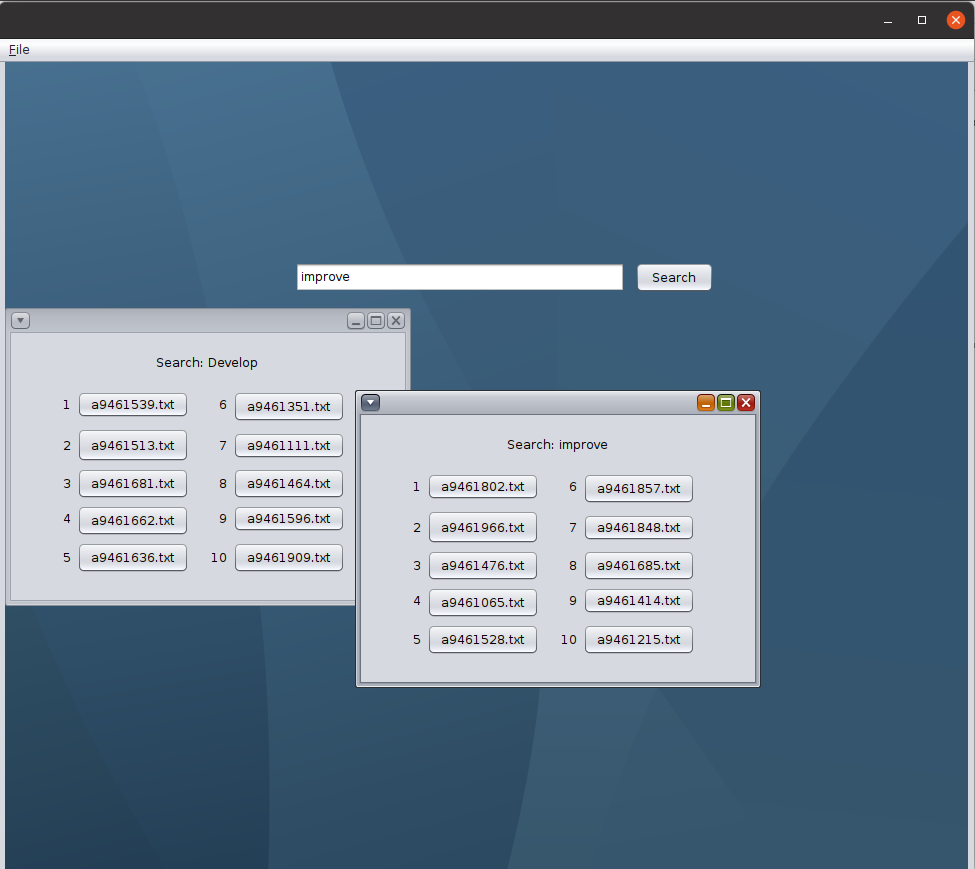
\includegraphics[width=0.7\linewidth]{Imagenes/screenshot007}
	\label{fig:screenshot007}
\end{figure}

Por último, podemos acceder al documento deseado pinchando en el botón de su nombre:

\begin{figure}[H]
	\centering
	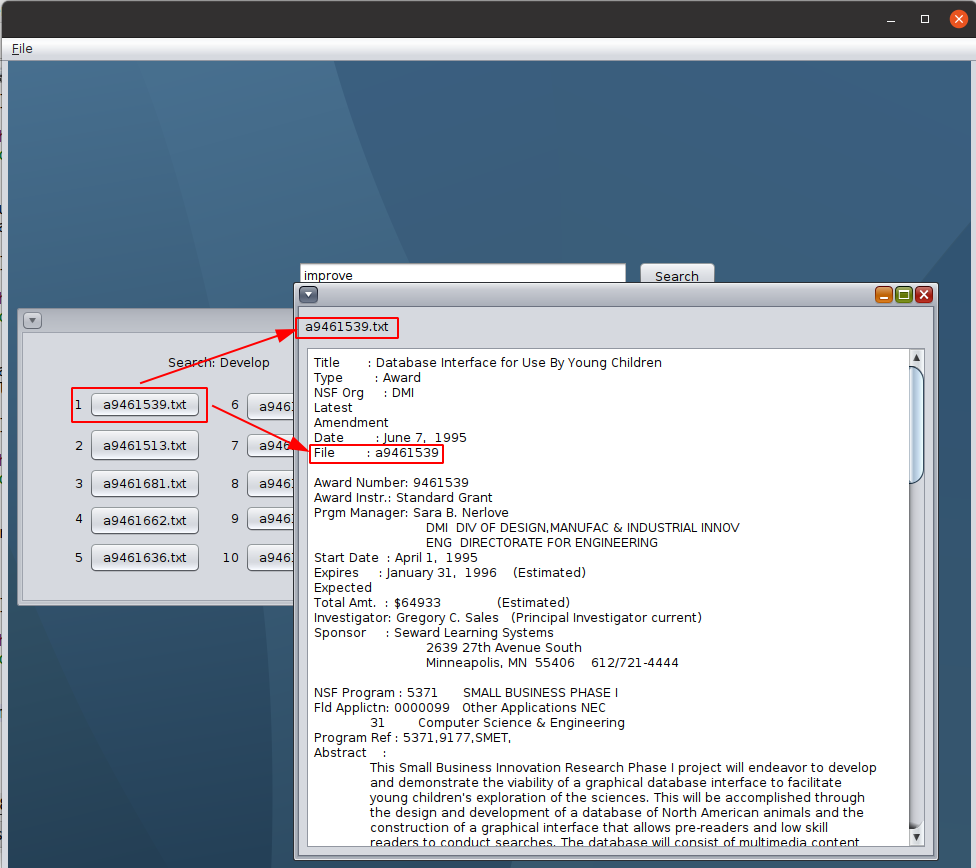
\includegraphics[width=0.7\linewidth]{Imagenes/screenshot008}
	\label{fig:screenshot008}
\end{figure}

Y con esto, llegamos al fin de la práctica realizada.

\section{Bibliografía consultada}
Además de basarme en la propia práctica, he usados estos dos tutoriales:

\url{https://www.ionos.es/digitalguide/servidores/configuracion/apache-lucene/}

\url{https://www.tutorialspoint.com/lucene/lucene_sorting.htm}

\url{https://lucene.apache.org/core/3_5_0/api/core/org/apache/lucene/search/IndexSearcher.html}

\url{https://www.jitendrazaa.com/blog/java/generating-executable-jar-file-with-all-dependencies-and-libraries-in-single-jar-using-netbeans-and-eclipse/}

\section{Enlace al fichero con los documentos}

\url{https://drive.google.com/drive/folders/1S9lbNau6TiDt-Xv2UnfUlgE94jQ3FzTh?usp=sharing}

\end{document}